\documentclass[../Hovedrapport.tex]{subfiles}
    \begin{document}
%--------------------------------------------------------------------------

%--------------------------------------------------------------------------
\section{Anlægsbeskrivelse  (Alle)}
    \label{sec:anlaegsbeskrivelse}
    % Følgende skal være med i dette afsnit.
    %	Et afsnit med titlen: ”Projektbeskrivelse”. Her skal der i tekst, figurer mv. være en så detaljeret beskrivelse af, hvad projektet går ud på – så en udenforstående kan få et nogenlunde overblik, og så vejlederen kan bedømme, om projektet kan indfri læringsmålene.
Et køleskab er et køleanlæg, som har til formål at fjerne varme fra et afgrænset rum og afgive denne til omgivelserne ved en højere temperatur. Et køleskab består overordnet set af to sider, hvorigennem der forgår varmeudveksling; en lavtryksside, inde i køleskabet og en højtryksside, uden på køleskabet. 

På lavtrykssiden befinder sig en varmeveksler i form af en fordamper, som har til formål at optage varmen fra luften samt mad- og drikkevarer i køleskabet. Dette er muligt, idet en fordamper udnytter princippet om, at en faseovergang fra væske til gas (fordampning) kræver en stor energitilførsel fra omgivelserne. Dette medfører en nedkøling af køleskabets indhold.

På højtrykssiden befinder sig en varmeveksler, i form af en kondensator, som har til formål at afgive den optagne varme fra køleskabets indhold til omgivelserne ved en højere temperatur. Dette er muligt, idet en kondensator udnytter princippet om, at en faseovergang fra gas til væske (kondensering) afgiver en stor mængde energi til omgivelserne i form af varme.

Køleanlægget drives af en kompressor, som befinder sig mellem fordamperen og kondensatoren. Kompressoren udfører et mekanisk arbejde på kølemidlet i kølekredsen, som bidrager til at øge kølemidlets tryk og dugpunktstemperatur. Kølemidlet gennemløber en ekspansionsventil, efter det har passeret kondensatoren, hvorved trykket falder. Dette medfører, at dugpunktstemperaturen falder, således at kølemidlet vil undergå en faseovergang fra væske til gas inde i fordamperen.

I dette anlæg vil fordamperen være placeret inde i en flamingokasse for at simulere et køleskab. Qua ovenstående kredsproces vil fordamperen optage varmeenergi inde i køleskabet, hvorefter denne energi afgives til omgivelserne via kondensatoren. Overordnet set vil der være en flytning af energi fra køleskab til det omgivende miljø, som i sidste ende medfører en nedkøling af drikke- og eventuelle madvarer. 
%--------------------------------------------------------------------------------
\subsection{Udvælgelse af typer af komponenter}
I dette afsnit identificeres hvilke komponenter, som bør anvendes til konstruktionen af køleanlægget. Herefter redegøres der, for hvilke krav der stilles til komponenterne og hvilke valgmuligheder, der er i forhold til komponenttyper. Endelig besluttes det, hvilke komponenter, som vil blive anvendt i køleanlægget.
%--------------------------------------------------------------------------------
\subsubsection*{Krav til komponenterne}
\label{sec:udv_komponenter}
Der er fire hovedkomponenter i køleanlægget, som skal udvælges. \\ 
Henholdsvis:
\begin{itemize}
    \item Kompressor
    \item Kondensator
    \item Ekspansionsventil
    \item Fordamper
\end{itemize}
Det er vigtigt, at komponenterne har den rigtige størrelse og kapacitet i forhold til eksempelvis den ønskede kuldeydelse. Her er det bl.a. væsentligt, at kompressoren bliver valgt med den rigtige størrelse, så den ikke bliver underdimensioneret, og derved ikke kan opnå den ønskede kuldeydelse. Kompressoren skal omvendt heller ikke overdimensioneres, således kølemidlet ikke kan nå at fordampe inden kompressoren. Ved udvælgelsen af kondensatoren er det vigtigt, at dens kapacitet er tilstrækkelig stor til at afgive varmeydelsen fra kølemidlet, så kølemidlet kondenserer tilbage på væskeform inden ekspansionsventilen. Ventilen skal udvælges således, at der opnås det ønskede tryktab over komponenten ved den givne kuldeydelse og massestrøm. Til sidst skal fordamperen udvælges således, at den fysisk kan være i køleskabet og kan optage den varme fra køleskabet, som svarer til kompressorens kølekapacitet.
%--------------------------------------------------------------------------------
\subsubsection*{Muligheder}
Der er forskellige muligheder i forhold til valg af kompressortype. Den ønskede kuldeydelse, type af kompressor, hvilket kølemiddel, der skal benyttes samt procesværdier er alle afgørende parametre for kompressoren. Ved procesværdier forstås kondenserings- og fordampningstemperaturen, overhedning og underkøling samt trykket på lav- og højtrykssiden af anlægget. Kompressorer optræder i typerne AC og DC, hvortil der skal vælges mellem en af disse to typer. \\
Når fordamperen og kondensatoren skal udvælges, skal disses kulde- og varmeydelse naturligvis bestemmes. Foruden dette skal det også besluttes, hvilken type varmeveksler, der skal anvendes i anlægget. Her kan der vælges mellem væske til væske, væske til gas eller gas til gas. Der skal ydermere tages stilling til, om fluidstrømningen omkring varmevekslerne skal ske ved fri konvektion eller ved tvungen luftstrømning. Endelig skal ventilen udvælges, hvor der her kan vælges mellem eksempelvis en ekspansionsventil eller et kapilarrør, hvor størrelsen af disse ligeledes skal bestemmes.
%--------------------------------------------------------------------------------
\subsubsection*{Beslutning}
Til køleanlægget udvælges en hermetisk DC-stempelkompressor. Kompressoren vælges som DC kompatibel, da dette gør det nemmere at omdrejningsregulere vha. en PID-regulering. Dette er et krav til kompressoren (jf. afsnit \ref{sec:kravspec}). En PID-omdrejningsregulering af kompressoren er ønsket, da det muliggør opretholdelsen af en stabil indvendig temperatur. Temperaturudsving betragtes ikke som værende fordelagtige for eventuelle fødevarer i køleskabet, da dette udtørrer disse. Ved en DC-kompressor er det nemmere at regulere omdrejningstallet end ved en AC-kompressor, hvilket skyldes, at en AC-kompressor skal omdrejningsreguleres vha. en frekvensregulering. En hermetisk stempelkompressor betegner, at motoren og kompressoren er i samme enhed, og dette sikrer en mere simpel anordning, som fylder mindre. For kompressoren er det også vigtigt, at den har kapaciteten til at sikre massestrømmen og trykforholdet til den ønskede kulde- eller varmeydelse. Ved udvælgelsen af fordamper og kondensator vælges der væske til gas varmevekslere i begge tilfælde. Dette betragtes som værende den simpleste konstruktion, da fluiden omkring begge varmevekslere vil være atmosfærisk luft. Foruden dette vælges det også, at luften, der strømmer henover varmevekslerne, skal være tvungen med en ventilator. Fordamperen ønskes ventileret, da dette sikrer en bedre varmeoveførsel mellem kølemiddel og luft, som medfører at en mindre varmeveksler kan benyttes. Den tvungne luftstrøm bevirker samtidig til en hurtigere nedkøling af drikkevarerne og sikrer ligeledes, at der en bedre luftcirkulation og fordeling af kølig luft indvendigt i køleskabet. 

Kondensatoren ønskes også ventileret, da dette sikrer en bedre varmeoverførsel til luften og dermed gør varmeveksleren mere kompakt. Dette ønskes stik imod konventionelle køleskabe, hvor kondensatoren er et rørbundt, som fylder hele bagsiden af køleskabet. Der er her risiko for, at bagsiden kan blive meget varm på konventionelle køleskabe grundet en mangel på fjernelse af varmen, hvilket også forværres, hvis bagsiden står i et indelukket rum.

Til sidst udvælges en ekspansionsventil, som kan sikre det nødvendige trykfald ved den ønskede kuldeydelse. En ekspansionsventil vælges fremfor et kapillarrør, idet en omdrejningsregulering af kompressoren ikke er kompatibel med et kapillarrør.

Komponenterne indsat fremgår af nedenstående figur \ref{fig:Anlægsoversigt}
% Figur:
\begin{figure}[H] % (alternativt [H])
	\centering
	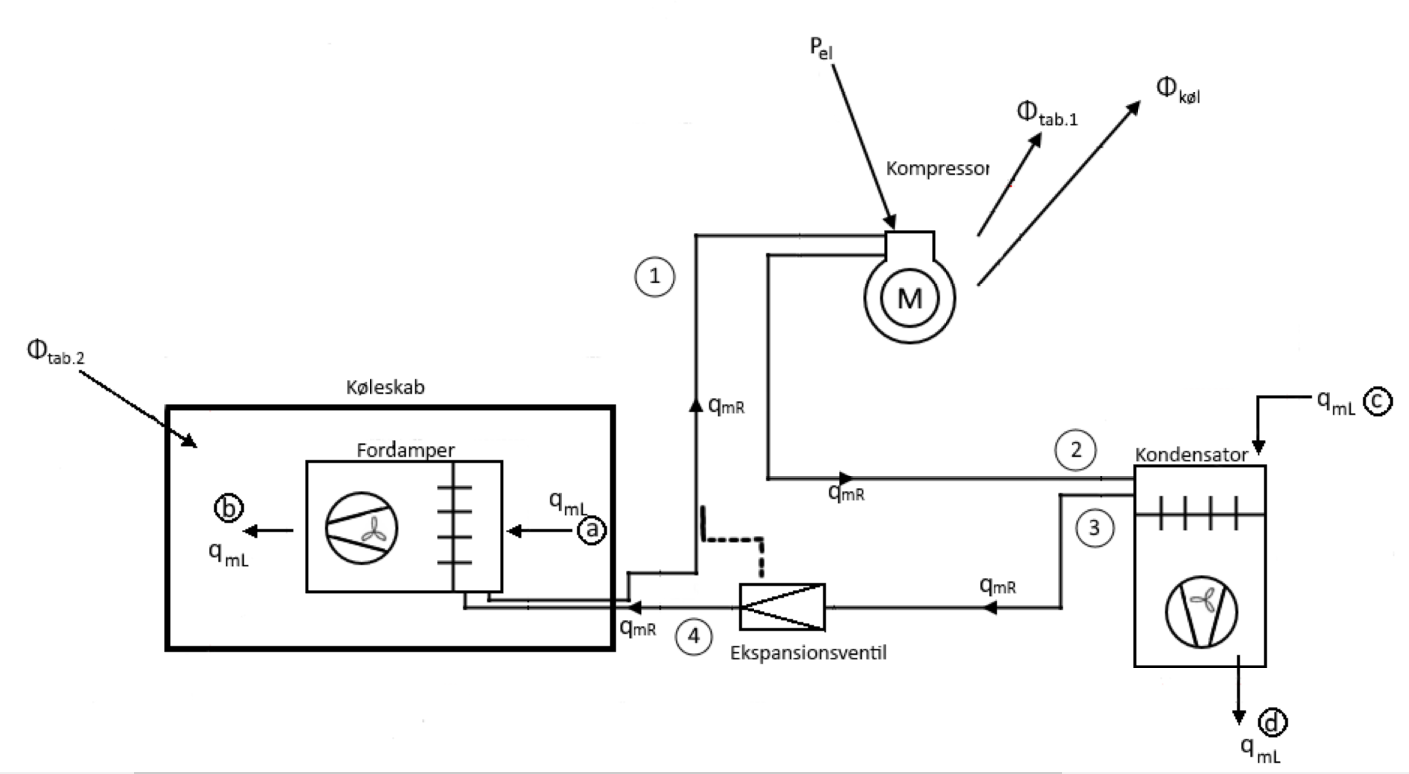
\includegraphics[width=1\textwidth]{Billeder/uden_KF.png}
	\caption{\textit{Oversigt over køleanlægget}.}
	\label{fig:Anlægsoversigt}
\end{figure}
%--------------------------------------------------------------------------------
\end{document}